% !TEX TS-program = knitr
\documentclass[handout]{beamer}\usepackage{graphicx, color}
%% maxwidth is the original width if it is less than linewidth
%% otherwise use linewidth (to make sure the graphics do not exceed the margin)
\makeatletter
\def\maxwidth{ %
  \ifdim\Gin@nat@width>\linewidth
    \linewidth
  \else
    \Gin@nat@width
  \fi
}
\makeatother

\IfFileExists{upquote.sty}{\usepackage{upquote}}{}
\definecolor{fgcolor}{rgb}{0.2, 0.2, 0.2}
\newcommand{\hlnumber}[1]{\textcolor[rgb]{0,0,0}{#1}}%
\newcommand{\hlfunctioncall}[1]{\textcolor[rgb]{0.501960784313725,0,0.329411764705882}{\textbf{#1}}}%
\newcommand{\hlstring}[1]{\textcolor[rgb]{0.6,0.6,1}{#1}}%
\newcommand{\hlkeyword}[1]{\textcolor[rgb]{0,0,0}{\textbf{#1}}}%
\newcommand{\hlargument}[1]{\textcolor[rgb]{0.690196078431373,0.250980392156863,0.0196078431372549}{#1}}%
\newcommand{\hlcomment}[1]{\textcolor[rgb]{0.180392156862745,0.6,0.341176470588235}{#1}}%
\newcommand{\hlroxygencomment}[1]{\textcolor[rgb]{0.43921568627451,0.47843137254902,0.701960784313725}{#1}}%
\newcommand{\hlformalargs}[1]{\textcolor[rgb]{0.690196078431373,0.250980392156863,0.0196078431372549}{#1}}%
\newcommand{\hleqformalargs}[1]{\textcolor[rgb]{0.690196078431373,0.250980392156863,0.0196078431372549}{#1}}%
\newcommand{\hlassignement}[1]{\textcolor[rgb]{0,0,0}{\textbf{#1}}}%
\newcommand{\hlpackage}[1]{\textcolor[rgb]{0.588235294117647,0.709803921568627,0.145098039215686}{#1}}%
\newcommand{\hlslot}[1]{\textit{#1}}%
\newcommand{\hlsymbol}[1]{\textcolor[rgb]{0,0,0}{#1}}%
\newcommand{\hlprompt}[1]{\textcolor[rgb]{0.2,0.2,0.2}{#1}}%

\usepackage{framed}
\makeatletter
\newenvironment{kframe}{%
 \def\at@end@of@kframe{}%
 \ifinner\ifhmode%
  \def\at@end@of@kframe{\end{minipage}}%
  \begin{minipage}{\columnwidth}%
 \fi\fi%
 \def\FrameCommand##1{\hskip\@totalleftmargin \hskip-\fboxsep
 \colorbox{shadecolor}{##1}\hskip-\fboxsep
     % There is no \\@totalrightmargin, so:
     \hskip-\linewidth \hskip-\@totalleftmargin \hskip\columnwidth}%
 \MakeFramed {\advance\hsize-\width
   \@totalleftmargin\z@ \linewidth\hsize
   \@setminipage}}%
 {\par\unskip\endMakeFramed%
 \at@end@of@kframe}
\makeatother

\definecolor{shadecolor}{rgb}{.97, .97, .97}
\definecolor{messagecolor}{rgb}{0, 0, 0}
\definecolor{warningcolor}{rgb}{1, 0, 1}
\definecolor{errorcolor}{rgb}{1, 0, 0}
\newenvironment{knitrout}{}{} % an empty environment to be redefined in TeX

\usepackage{alltt}

\setbeamercovered{dynamic}
\usetheme{Marburg}
\setbeamertemplate{navigation symbols}{} 
\setbeamertemplate{footline}
{
  \leavevmode%
  \hbox{%
  \begin{beamercolorbox}[wd=.333333\paperwidth,ht=2.25ex,dp=1ex,center]{author in head/foot}%
    \usebeamerfont{author in head/foot}\copyright $\ $ \insertshortauthor%~~\beamer@ifempty{\insertshortinstitute}{}{(\insertshortinstitute)}
  \end{beamercolorbox}%
  \begin{beamercolorbox}[wd=.333333\paperwidth,ht=2.25ex,dp=1ex,center]{title in head/foot}%
    \usebeamerfont{title in head/foot} \insertinstitute
  \end{beamercolorbox}%
  \begin{beamercolorbox}[wd=.333333\paperwidth,ht=2.25ex,dp=1ex,right]{date in head/foot}%
    \usebeamerfont{date in head/foot}\insertshortdate{}\hspace*{2em}
    \insertframenumber{} / \inserttotalframenumber\hspace*{2ex} 
  \end{beamercolorbox}}%
  \vskip0pt%
}

\usepackage{amsmath}
\usepackage{caption}
\usepackage{color}
\usepackage{enumerate}
\usepackage{listings}
\usepackage{hyperref}
\usepackage{mathrsfs}
\usepackage{natbib}
\usepackage{soul}
\usepackage{ulem}
\usepackage{hyperref}
\usepackage{url}


\providecommand{\all}{\ \forall \ }
\providecommand{\bs}{\backslash}
\providecommand{\e}{\varepsilon}
\providecommand{\E}{\ \exists \ }
\providecommand{\lm}[2]{\lim_{#1 \rightarrow #2}}
\providecommand{\m}[1]{\mathbb{#1}}
\providecommand{\nv}{{}^{-1}}
\providecommand{\ov}[1]{\overline{#1}}
\providecommand{\p}{\newpage}
\providecommand{\q}{$\quad$ \newline}
\providecommand{\rt}{\rightarrow}
\providecommand{\Rt}{\Rightarrow}
\providecommand{\vc}[1]{\boldsymbol{#1}}
\providecommand{\wh}[1]{\widehat{#1}}

\hypersetup{colorlinks,linkcolor=,urlcolor=blue}
\numberwithin{equation}{section}

\definecolor{dkgreen}{rgb}{0,0.6,0}
\definecolor{gray}{rgb}{0.5,0.5,0.5}
\definecolor{mauve}{rgb}{0.58,0,0.82}

\lstset{ 
  language=C,                % the language of the code
  basicstyle= \footnotesize,           % the size of the fonts that are used for the code
  numberstyle= \tiny \color{white},  % the style that is used for the line-numbers
  stepnumber=2,                   % the step between two line-numbers. 
  numbersep=5pt,                  % how far the line-numbers are from the code
  backgroundcolor=\color{white},      % choose the background color. You must add \usepackage{color}
  showspaces=false,               % show spaces adding particular underscores
  showstringspaces=false,         % underline spaces within strings
  showtabs=false,                 % show tabs within strings adding particular underscores
  frame=lrb,                   % adds a frame around the code
  rulecolor=\color{black},        % if not set, the frame-color may be changed on line-breaks within not-black text 
  tabsize=2,                      % sets default tabsize to 2 spaces
  captionpos=t,                   % sets the caption-position 
  breaklines=true,                % sets automatic line breaking
  breakatwhitespace=false,        % sets if automatic breaks should only happen at whitespace
  %title=\lstname,                   % show the filename of files included with \lstinputlisting;
  keywordstyle=\color{blue},          % keyword style
  commentstyle=\color{gray},       % comment style
  stringstyle=\color{dkgreen},         % string literal style
  escapeinside={\%*}{*)},            % if you want to add LaTeX within your code
  morekeywords={*, ...},               % if you want to add more keywords to the set
  xleftmargin=0.053in, % left horizontal offset of caption box
  xrightmargin=-.03in % right horizontal offset of caption box
}

%\DeclareCaptionFont{white}{\color{white}}
%\DeclareCaptionFormat{listing}{\parbox{\textwidth}{\colorbox{gray}{\parbox{\textwidth}{#1#2#3}}\vskip-0.05in}}
%\captionsetup[lstlisting]{format = listing, labelfont = white, textfont = white}
%For caption-free listings, comment out the 3 lines above and uncomment the 2 lines below.
 \captionsetup{labelformat = empty, labelsep = none}
 \lstset{frame = single}




\title{Special Discrete Random Variables (Ch. 5.1)}
\author{Will Landau}
\date{Feb 19, 2013}
\institute{Iowa State University}

\begin{document}

\begin{frame}
\titlepage
 \end{frame}
 
 \AtBeginSection[]
{
   \begin{frame}
       \frametitle{Outline}
       \tableofcontents[currentsection]
   \end{frame}
}

\section{Binomial Distribution}


\begin{frame}
\frametitle{The Binomial Distribution}
\begin{itemize}
\pause \item $X \sim$ Binomial($n$, $p$) $-$ i.e., $X$ is distributed as a binomial random variable with parameters $n$ and $p$ ($0 < p < 1)$ if:
\pause \begin{align*}
f_X(x) = 
\begin{cases}
\binom{n}{x} p^x (1-p)^{n-x} & x = 0, \ldots, n\\
0 & \text{otherwise} 
\end{cases}
\end{align*}
where: 
\begin{itemize}
\pause \item $\binom{n}{x} = \frac{n!}{x!(n-x)!}$, read ``$n$ choose $x$"
\pause \item $n!$ = $n \cdot (n-1) \cdot \cdots \cdot 2 \cdot 1$, the factorial function.
\end{itemize}
\pause \item $E(X) = np$
\pause \item $Var(X) = np(1-p)$
\end{itemize}
\end{frame}

\begin{frame}
\frametitle{The Binomial Distribution}
\setkeys{Gin}{width=1\textwidth} 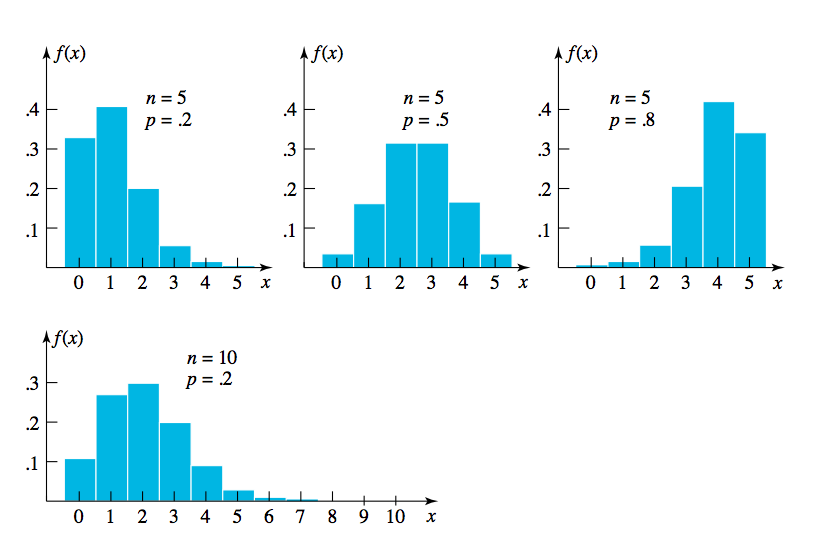
\includegraphics{../../fig/binombar.png}
\end{frame}

\begin{frame}
\frametitle{Purpose of the binomial random variable}
\begin{itemize}
\item  A Bin($n$, $p$) random variable counts the number of successes in $n$ success-failure trials that:
\begin{itemize}
\pause \item are independent of one another.
\pause \item each succeed with probability $p$.
\end{itemize}
\pause \item Examples:
\begin{itemize}
\pause \item Number of conforming hexamine pellets in a batch of $n = 50$ total pellets made from a pelletizing machine.
\pause \item Number of runs of the same chemical process with percent yield above 80\%, given that you run the process a total of $n = 1000$ times.
\pause \item Number of rivets that fail in a boiler of $n = 25$ rivets within 3 years of operation. (Note; ``success" doesn't always have to be good.)
\end{itemize}
\end{itemize}
\end{frame}

\begin{frame}
\frametitle{Example: machine with 10 components}
\begin{center}
\setkeys{Gin}{width=1\textwidth} 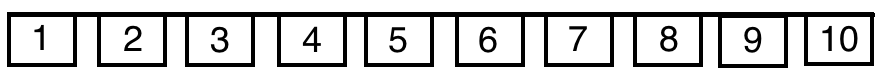
\includegraphics{../../fig/mach1.png}
\end{center}
\begin{itemize}
\pause \item Suppose you have a machine with 10 {\bf independent} components in series. The machine only works if all the components work.
\pause \item Each component succeeds with probability $p = 0.95$ and fails with probability $1 - p = 0.05$.  \
\pause \item Let $Y$ be the number of components that succeed in a given run of the machine. Then:
\begin{align*}
Y \sim \text{Binomial}(n = 10, p = 0.95)
\end{align*}
\end{itemize}

\end{frame}

\begin{frame}
\frametitle{Example: machine with 10 components}
\begin{align*}
\uncover<2->{P(\text{machine succeeds})} &\uncover<2->{= P(Y = 10)} \\
&\uncover<3->{= \binom{10}{10}p^{10} (1-p)^{10 - 10}} \\
&\uncover<4->{= p^{10}} \\
&\uncover<5->{=0.95^{10}} \\
&\uncover<6->{= 0.5987}
\end{align*}
\begin{itemize}
\uncover<7->{\item This machine isn't very reliable.}
\end{itemize}
\end{frame}

\begin{frame}
\frametitle{Example: machine with 10 components}

\begin{center}
\setkeys{Gin}{width=1\textwidth} 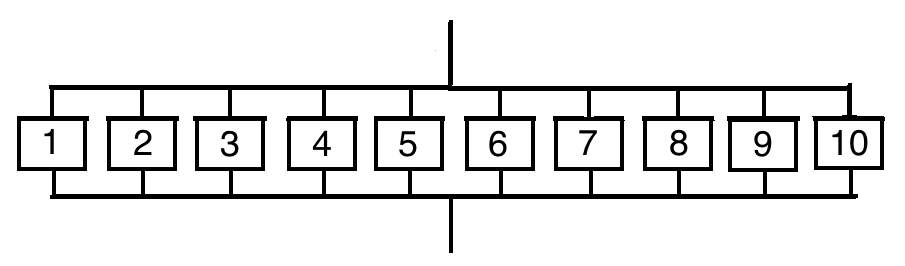
\includegraphics{../../fig/mach3.png}
\end{center}

\begin{itemize}
\pause \item What if I arrange these 10 components in parallel? This machine succeeds if at least 9 of the components succeed.
\pause \item What is the probability that the new machine succeeds?
\end{itemize}


\end{frame}


\begin{frame}
\frametitle{Example: machine with 10 components}

\begin{align*}
&\uncover<2->{P(\text{improved machine succeeds)}} \\
& \qquad \uncover<2->{= P(Y \ge 9)} \\
&\qquad \uncover<3->{= P(Y = 9) + P(Y = 10)} \\
&\qquad  \uncover<4->{=\binom{10}{9}p^9 (1-p) + \binom{10}{10} p^{10} (1-p)^{10 - 10}} \\
&\qquad \uncover<5->{=(10) \cdot 0.95^9 \cdot 0.05 + (1) \cdot 0.95^{10}} \\
&\qquad \uncover<6->{= 0.9139}
\end{align*}
\begin{itemize}
\uncover<7->{\item By allowing just one component to fail, we made this machine far more reliable.}
\end{itemize}

\end{frame}\begin{frame}
\frametitle{Example: machine with 10 components}
\begin{itemize}
\item If we allow up to 2 components to fail:
\end{itemize}
\small
\begin{align*}
&\uncover<2->{P(\text{improved machine succeeds)}} \\
& \quad \uncover<2->{= P(Y \ge 8)} \\
&\quad \uncover<3->{= P(Y = 8) + P(Y = 9) + P(Y = 10)} \\
&\quad  \uncover<4->{=\binom{10}{8} p^8 (1-p)^{10 - 8} + \binom{10}{9}p^9 (1-p) + \binom{10}{10} p^{10} (1-p)^{10 - 10}} \\
&\quad \uncover<5->{=\frac{10!}{(10-8)!8!} \cdot 0.95^8 \cdot 0.05^2 + (10) \cdot 0.95^9 \cdot 0.05 + (1) \cdot 0.95^{10}} \\
&\quad \uncover<6->{= 0.9885}
\end{align*}


\end{frame}
\begin{frame}
\frametitle{Example: machine with 10 components}

\begin{itemize}
 \item $E(Y) = np = 10 \cdot 0.95 = 9.5$. So the number of components to fail per run on average is 9.5.
\pause \item $Var(Y) = np(1-p) = 10 \cdot 0.95 \cdot (1- 0.95) = 0.475$.
\pause \item $SD(Y) = \sqrt{Var(Y)} = \sqrt{np(1-p)}  =0.689$. 
\end{itemize}

\end{frame}



\section{Geometric Distribution}



\begin{frame}
\frametitle{Geometric random variables}

\begin{itemize}
\uncover<2->{ \item $X \sim $ Geometric($p$) $-$ that is, $X$ has a geometric distribution with parameter $p$ ($0 < p < 1$) $-$ if its pmf is:}
\begin{align*}
\uncover<3->{ f_X(x)} & \uncover<3->{= \begin{cases}
p(1-p)^{x - 1} & x = 1, 2, 3, \ldots \\
0 & \text{otherwise}
\end{cases} }
\intertext{\uncover<4->{ and its cdf is:}}
\uncover<5->{ F_X(x)} & \uncover<5->{= \begin{cases}
1-(1-p)^{x} & x = 1, 2, 3, \ldots \\
0 & \text{otherwise}
\end{cases} }
\end{align*}
\uncover<6->{ \item $E(X) = \frac{1}{p}$}
\uncover<7->{ \item $Var(X) = \frac{1-p}{p^2}$}
\end{itemize}
\end{frame}

\begin{frame}
\frametitle{A look at the Geom($p$) distribution}
\begin{center}
\setkeys{Gin}{width=.7\textwidth} 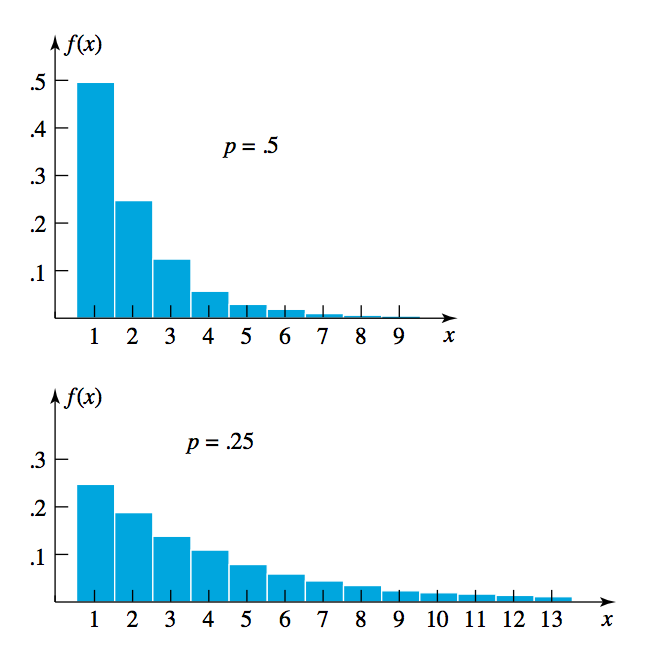
\includegraphics{../../fig/geombar.png}
\end{center}
\end{frame}


\begin{frame}
\frametitle{Uses of the $X \sim$ Geom($p$)}
\begin{itemize}
\pause \item For an indefinitely-long sequence of independent, success-failure trials, each with P(success) = $p$, $X$ is the number of trials it takes to get a success.
\pause \item Examples:
\begin{itemize}
\pause \item Number of rolls of a fair die until you land a 5.
\pause \item Number of shipments of raw material you get until you get a defective one.
\pause \item The number of enemy aircraft that fly close before one flies into friendly airspace.
\pause \item Number hexamine pellets you make before you make one that does not conform.
\pause \item Number of buses that come before yours.
\end{itemize}
\end{itemize}
\end{frame}


\begin{frame}
\frametitle{Example: shorts in NiCad batteries} \scriptsize

\begin{itemize}
\uncover<2->{ \item An experimental program was successful in reducing the percentage of manufactured NiCad cells with internal shorts to around 1\%. }
\uncover<3->{  \item Let $T$ be the test number at which the first short is discovered. Then, $T \sim $ Geom($p$).}
\end{itemize}

\begin{align*}
\uncover<4->{ P(\text{1st or 2nd cell tested is has the 1st short})} &\uncover<4->{ = P(T = 1 \text{ or } T = 2)} \\
&\uncover<5->{  = f(1) + f(2)} \\
&\uncover<6->{  = p + p(1-p)} \\
&\uncover<7->{  = 0.01 + 0.01 (1 - 0.01)} \\
&\uncover<8->{  = 0.02}
\end{align*}

\begin{align*}
\uncover<9->{ P(\text{at least 50 cells tested w/o finding a short})} &\uncover<9->{ = P(T > 50)} \\
&\uncover<10->{  = 1 - P(T \le 50)} \\
&\uncover<11->{  = 1 - F(50) }\\
&\uncover<12->{  = 1 - (1 - (1-p)^x)} \\
&\uncover<13->{  = (1-p)^x} \\
& \uncover<14->{ = (1 - 0.01)^{50}} \\
&\uncover<15->{  = 0.61}
\end{align*}
\end{frame}


\begin{frame}
\frametitle{Example: shorts in NiCad batteries}
\begin{align*}
\uncover<2->{E(T)} & \uncover<2->{ = \frac{1}{p} = \frac{1}{0.01}} \\
&\uncover<3->{ = 100 \text{ tests for the first short to appear, on avg.}} \\
\uncover<4->{ SD(T)} &\uncover<4->{ = \sqrt{Var(T)} = \sqrt{\frac{1-p}{p^2}}} \\
& \uncover<5->{=  \sqrt{\frac{1-0.01}{0.01^2}} = 99.5 \text{ tested batteries}}
\end{align*}
\end{frame}






\section{ Poisson Distribution}


\begin{frame}
\frametitle{Poisson random variables}
\begin{itemize}
\pause \item $X \sim $ Poisson($\lambda$) $-$ that is, $X$ has a geometric distribution with parameter $\lambda > 0$ $-$ if its pmf is:
\pause \begin{align*}
f_X(x) = \begin{cases}
\frac{e^{-\lambda}\lambda^x}{x!} & x = 0,1 , 2, 3, \ldots \\
0 & \text{otherwise}
\end{cases}
\end{align*}
\pause \item $E(X) = \lambda$
\pause \item $Var(X) = \lambda$
\end{itemize}
\end{frame}

\begin{frame}
\frametitle{A look at the Poisson distribution}
\begin{center}
\setkeys{Gin}{width=.7\textwidth} 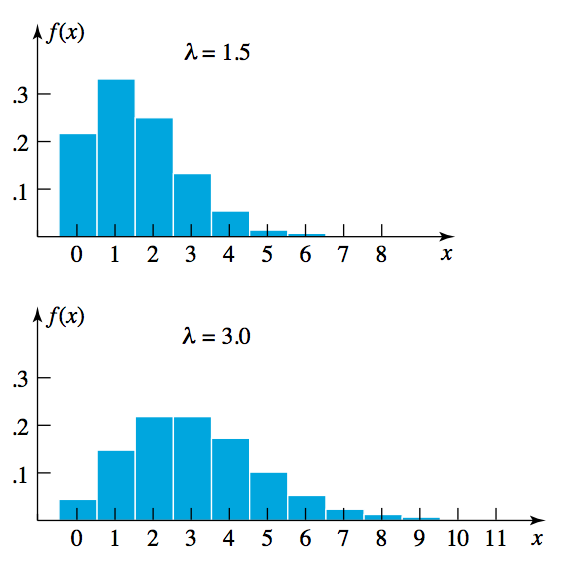
\includegraphics{../../fig/poissonbar.png}
\end{center}
\end{frame}

\begin{frame}
\frametitle{Meaning of the Poisson distribution}
\begin{itemize}
\pause \item A Poisson($\lambda$) random variable counts the number of occurrences that happen over a fixed interval of time or space.
\pause \item These occurrences must:
\begin{itemize}
\pause \item be independent
\pause \item be sequential in time (no two occurrences at once)
\pause \item occur at the same constant rate, $\lambda$.
\end{itemize}
\pause \item $\lambda$, the {\bf rate parameter}, is the expected number of occurrences in the specified interval of time or space.
\end{itemize}
\end{frame}


\begin{frame}
\frametitle{Examples} \small
\begin{itemize}
\pause \item $Y$ is the number of shark attacks off the coast of CA next year. $\lambda = 100$ attacks per year.
\pause \item $Z$ is the number of shark attacks off the coast of CA next month. $\lambda = 100/12 = 8.3333$ attacks per month
\pause \item $N$ is the number of $\beta$ particles emitted from a small bar of plutonium, registered by a Geiger counter, in a minute. $\lambda$ = 459.21 particles/minute.
\pause \item $J$ is the number of particles per three minutes. $\lambda = $?
\begin{align*}
\uncover<6->{\lambda} &\uncover<6->{= \frac{459.21 \text{ (units particle)}}{1 {\text{ (unit minute)}}}} \uncover<7->{\cdot \frac{3 {\text{ (units minute})}}{1 \text{ (unit of 3 minutes})}} \\
&\uncover<8->{= \frac{1377.63 \text{ (units particle)}}{1 \text{ (unit of 3 minutes)}}} \uncover<9->{= 1377.62 \text{ particles per 3 minutes}}
\end{align*}
\end{itemize}
\end{frame}

\begin{frame}
\frametitle{Example: Rutherford/Geiger experiment} \scriptsize
\begin{itemize}
\pause \item Rutherford and Geiger measured the number of $\alpha$ particles detected near a small bar of plutonium for 8-minute periods.
\pause \item The average number of particles per 8 minutes was $\lambda = 3.87$ particles / 8 min.
\pause \item Let $S \sim $ Poisson($\lambda$), the number of particles detected in the next 8 minutes. 
\end{itemize}
\begin{align*}
&\uncover<4->{f(s) = \begin{cases}
\frac{e^{-3.87}(3.87)^s}{s!} & \quad s = 0, 1, 2, \ldots \\
0 & \quad \text{otherwise}
\end{cases}} \\
&\uncover<5->{P(\text{at least 4 particles recorded})} \\
& \uncover<6->{\qquad = P(S \ge 4)} \\
& \uncover<7->{\qquad = f(4) + f(5) + f(6) + \cdots} \\
& \uncover<8->{\qquad = 1 - f(0) - f(1) - f(2) - f(3)} \\
& \uncover<9->{\qquad = 1 - \frac{e^{-3.87}(3.87)^0}{0!}  - \frac{e^{-3.87}(3.87)^1}{1!}} \\
& \uncover<9->{ \qquad \qquad  - \frac{e^{-3.87}(3.87)^2}{2!} - \frac{e^{-3.87}(3.87)^3}{3!}} \\
& \uncover<10->{\qquad = 0.54}
\end{align*}
\end{frame}

\begin{frame}
\frametitle{Example: arrival at a university library} \small
\begin{itemize}
\pause \item Some students' data indicate that between 12:00 and 12:10 P.M. on Monday through Wednesday, an average of around 125 students entered a library at Iowa State University library. 
\pause \item Let $M$ be the number of students entering the ISU library between 12:00 and 12:01 PM next Tuesday.
\pause \item Model $M \sim $ Poisson($\lambda$). 
\pause \item Having observed 125 students enter between 12:00 and 12:10 PM last Tuesday, we might choose:
\begin{align*}
&\uncover<5->{\lambda} = \uncover<5->{\frac{125 \text{ (units of student)}}{1 \text{ (unit of 10 minutes)}}} \uncover<6->{\cdot \frac{ \text{1 (unit of 10 minutes)}}{ \text{10 (units of minute)}}} \\
&\uncover<7->{=\frac{12.5 \text{ (units of student)}}{ \text{1 (unit minute)}}} \uncover<8->{= 12.5 \text{ students per minute}}
\end{align*}
\end{itemize}
\end{frame}

\begin{frame}
\frametitle{Example: arrival at a university library} \small
\begin{itemize}
\pause \item Under this model, the probability that between 10 and 15 students arrive at the library between 12:00 and 12:01 PM is:
\end{itemize}

\begin{align*}
&\uncover<3->{P(10 \le M \le 15)} \uncover<4->{= f(10) + f(11) + f(12) + f(13) + f(14) + f(15)} \\
& \qquad \uncover<5->{=\frac{e^{-12.5}(12.5)^{10}}{10!} + \frac{e^{-12.5}(12.5)^{11}}{11!} + \frac{e^{-12.5}(12.5)^{12}}{12!}} \\
&\qquad \uncover<5->{+\frac{e^{-12.5}(12.5)^{13}}{13!} + \frac{e^{-12.5}(12.5)^{14}}{14!} + \frac{e^{-12.5}(12.5)^{15}}{15!}} \\
&\qquad \uncover<6->{=0.60}
\end{align*}
\end{frame}


\begin{frame}
\frametitle{Example: shark attacks}
\begin{itemize}
\pause \item Let $X$ be the number of unprovoked shark attacks that will occur off the coast of Florida next year.
\pause \item Model $X \sim $ Poisson($\lambda$).
\pause \item From the shark data at \url{http://www.flmnh.ufl.edu/fish/sharks/statistics/FLactivity.htm}, 246 unprovoked shark attacks occurred from 2000 to 2009.
\pause \item Hence, I calculate:
\begin{align*}
\uncover<6->{\lambda} &\uncover<6->{= \frac{246 \text{ (units attack)}}{1 \text{ (unit of 10 years)}}} \uncover<7->{\cdot \frac{1 \text{ (unit of 10 years)}}{10 \text{ (units year)}}} \\
&\uncover<8->{=\frac{24.6 \text{ (units attack)}}{1 \text{(unit year)}}} \uncover<9->{= 24.6 \text{ attacks per year} }
\end{align*}
\end{itemize}
\end{frame}

\begin{frame}
\frametitle{Example: shark attacks} \small

\begin{align*}
&\uncover<2->{P(\text{no attacks next year}) \uncover<3->{=f(0)} \uncover<4->{= e^{-24.6} \cdot \frac{24.6^0}{0!}}} \\
&\uncover<5->{ \qquad \approx 2.07 \times 10^{-11}} \\
&\uncover<6->{P(\text{at least 5 attacks}) = 1 - P(\text{at most 4 attacks})} \\
&\uncover<7->{ \qquad =1 - F(4)} \\
&\uncover<8->{ \qquad =1 - f(0) - f(1) - f(2) - f(3) - f(4)} \\
&\uncover<9->{ \qquad =1 - e^{-24.6} \frac{24.6^0}{0!} - e^{-24.6} \frac{24.6^1}{1!} - e^{-24.6} \frac{24.6^2}{2!}} \\
&\uncover<9->{ \qquad - e^{-24.6} \frac{24.6^3}{3!} - e^{-24.6} \frac{24.6^4}{4!}} \\
&\uncover<10->{\qquad \approx 0.9999996} \\
&\uncover<11->{P(\text{more than 30 attacks}) = 1 - P(\text{at least 30 attacks})} \\
&\uncover<12->{ \qquad= 1 - e^{-24.6} \sum_{i = 0}^{30} \frac{24.6^x}{x!}}  \uncover<13->{= 1 - e^{-24.6} \cdot 4.251 \times 10^{10}} \\
&\uncover<14->{ \qquad \approx 0.1193}
\end{align*}
\end{frame}

\begin{frame}
\frametitle{Example: shark attacks}
\begin{itemize}
\pause \item Now, let $Y$ be the total number of shark attacks in Florida during the next 4 months.
\pause \item Let $Y \sim $ Poisson($\theta$), where $\theta$ is the true shark attack rate per 4 months:
\begin{align*}
\uncover<4->{\theta} &\uncover<4->{= \frac{24.6 \text{ (units attack)}}{1 \text{ (unit year)}}} \uncover<5->{ \cdot \frac{1/3 \text{ (unit year)}}{1 \text{ (unit of 4 months)}}} \\
& \uncover<6->{= \frac{8.2 \text{ (units attack)}}{1 \text{ (unit of 4 months)}}} \uncover<7->{ = 8.2 \text{ attacks per 4 months}}
\end{align*}
\end{itemize}
\end{frame}

\begin{frame}
\frametitle{Example: shark attacks} \small
\begin{align*}
&\uncover<2->{P(\text{no attacks next year}) \uncover<3->{=f(0)} \uncover<4->{= e^{-8.2} \cdot \frac{8.2^0}{0!}}} \\
&\uncover<5->{ \qquad \approx 0.000275} \\
&\uncover<6->{P(\text{at least 5 attacks}) = 1 - P(\text{at most 4 attacks})} \\
&\uncover<7->{ \qquad =1 - F(4)} \\
&\uncover<8->{ \qquad =1 - f(0) - f(1) - f(2) - f(3) - f(4)} \\
&\uncover<9->{ \qquad =1 - e^{-8.2} \frac{8.2^0}{0!} - e^{-8.2} \frac{8.2^1}{1!} - e^{-8.2} \frac{8.2^2}{2!}} \\
&\uncover<9->{ \qquad - e^{-8.2} \frac{8.2^3}{3!} - e^{-8.2} \frac{8.2^4}{4!}} \\
&\uncover<10->{\qquad \approx 0.9113} \\
&\uncover<11->{P(\text{more than 30 attacks}) = 1 - P(\text{at least 30 attacks})} \\
&\uncover<12->{ \qquad= 1 - e^{-8.2} \sum_{i = 0}^{30} \frac{8.2^x}{x!}} \uncover<13->{= 1 - e^{-8.2} \cdot 4.251 \times 10^{10}} \\
&\uncover<14->{ \qquad \approx 9.53 \times 10^{-10}}
\end{align*}
\end{frame}


\end{document}
